\section{Delta Squared‑DFT}
{{\footnotesize
\begin{description}[labelwidth=5em, labelsep=1em, leftmargin=*, align=left, itemsep=0.3em, parsep=0em]
  \item[date:] 2024-12-13
  \item[last\_updated:] 2024-12
  \item[expired:] unkown
  \item[valid:] yes
  \item[url:] \href{https://neurips.cc/virtual/2024/poster/97788}{https://neurips.cc/virtual/2024/poster/97788}
  \item[domain:] Computational Chemistry; Materials Science
  \item[focus:] Benchmarking machine-learning corrections to DFT using Delta Squared-trained models for reaction energies
  \item[keywords:]
    - density functional theory
    - Delta Squared‑ML correction
    - reaction energetics
    - quantum chemistry
  \item[task\_types:]
    - Regression
  \item[ai\_capability\_measured:]
    - High-accuracy energy prediction
    - DFT correction
  \item[metrics:]
    - Mean Absolute Error (eV)
    - Energy ranking accuracy
  \item[models:]
    - Delta Squared‑ML correction networks
    - Kernel ridge regression
  \item[ml\_motif:]
    - Scientific ML
  \item[type:] Dataset + Benchmark
  \item[ml\_task:] Regression
  \item[notes:] Demonstrates CC-level accuracy with \textasciitilde{}1\% of high-level data. Benchmarks publicly included for reproducibility.
  \item[contact.name:] Wei Liu
  \item[contact.email:] unkown
  \item[results.name:] ChatGPT LLM
  \item[results.url:] \href{unkown}{unkown}
  \item[fair.reproducible:] Yes
  \item[fair.benchmark\_ready:] Yes
  \item[ratings.software.rating:] 0
  \item[ratings.software.reason:] Not analyzed.
  \item[ratings.specification.rating:] 8.0
  \item[ratings.specification.reason:] Clear goals around unifying urban data formats and tasks (e.g., air quality prediction), though some specifics could be more formal.
  \item[ratings.dataset.rating:] 9.0
  \item[ratings.dataset.reason:] Multi-modal data is standardized and accessible; GitHub repo available.
  \item[ratings.metrics.rating:] 8.0
  \item[ratings.metrics.reason:] Uses common task metrics like accuracy/RMSE, though varies by task.
  \item[ratings.reference\_solution.rating:] 7.0
  \item[ratings.reference\_solution.reason:] Baseline regression/classification models included.
  \item[ratings.documentation.rating:] 8.0
  \item[ratings.documentation.reason:] Source code supports pipeline reuse, but formal evaluation splits may vary.
  \item[id:] delta\_squareddft
  \item[Citations:] \cite{khrabrov2024nabla2dftuniversalquantumchemistry}
  \item[Ratings:]
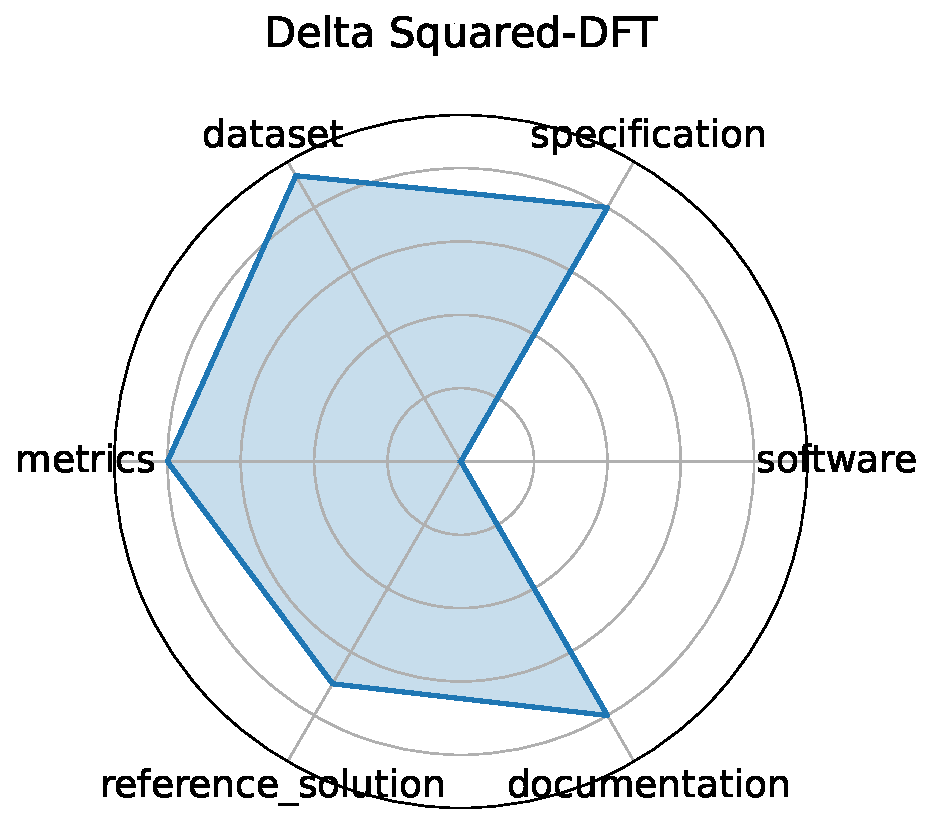
\includegraphics[width=0.2\textwidth]{delta_squareddft_radar.pdf}
\end{description}
}}
\clearpage